\subsection{Network analysis}

The network analysis proved very difficult. Mitmproxy was used to capture network traffic to and from the emulator. 
However, it required an SSL Certificate in order to capture encrypted traffic.
Sadly, since android version 7.x and up user installed SSL certificates are not trusted by default any longer.
The malicious application might also use certificate pinning to not allow any certificate but the specific one it specifies.
To bypass these issues an application called \href{https://github.com/shroudedcode/apk-mitm}{apk-mitm} was used to modify the malicious application to make it allow the SSL certificate mitmproxy used.
After a quick test, this seemed to work.

\subsubsection{HTTP proxy analysis}

Mitmproxy quickly revealed that requests were made to an API created by \href{https://telegram.org/}{telegram}.

The request in figure \ref{rafael-requesturl} was made to an endpoint for sending messages using a bot account. 
The documentation for the used endpoint can be found \href{https://core.telegram.org/method/messages.sendMessage}{here}.

The message sent can be seen in figure \ref{rafael-requestcontent}, it used some weird characters.
However, it was possible to read that it said \texttt{NEW DEVICE INSTALLED}.
The request also included a \texttt{chat\_id}, according to the documentation this parameter defined in what chat the message had to be sent.
This could for example send it to a specific user or a group chat.

The response can be seen in figure \ref{rafael-requestresponse}, it clarified that the message was still being sent, 
it was sent to a user with the name \texttt{L0gicMan} and the person sending the message had the username \texttt{logicmanBOT}.
The response also clarified that the message was \texttt{NEW DEVICE INSTALLED}

Figure \ref{rafael-requestlist} also shows that requests were also made to the \href{https://core.telegram.org/bots/api#getupdates}{getUpdates} endpoint.
This endpoint returned any new messages in a chat to the malicious application.
It never actually returned any useful data during testing.
Any other requests shown in this list were requests made by the Google Play Store.

\begin{figure}[H]
    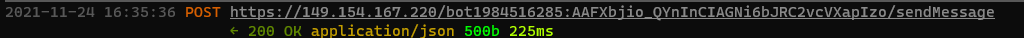
\includegraphics[width=1\textwidth]{postrequesturl.png}
    \caption{Request URL and method}
    \label{rafael-requesturl}
\end{figure}
\begin{figure}[H]
    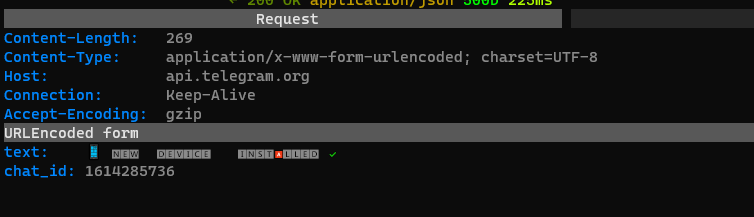
\includegraphics[width=1\textwidth]{postrequest.png}
    \caption{Request content}
    \label{rafael-requestcontent}
\end{figure}
\begin{figure}[H]
    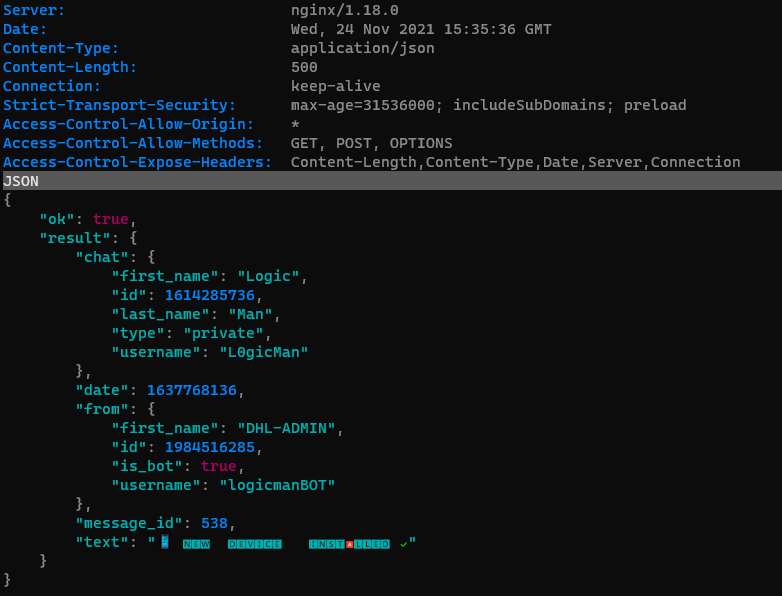
\includegraphics[width=1\textwidth]{postrequestresponse.png}
    \caption{Request response}
    \label{rafael-requestresponse}
\end{figure}
\begin{figure}[H]
    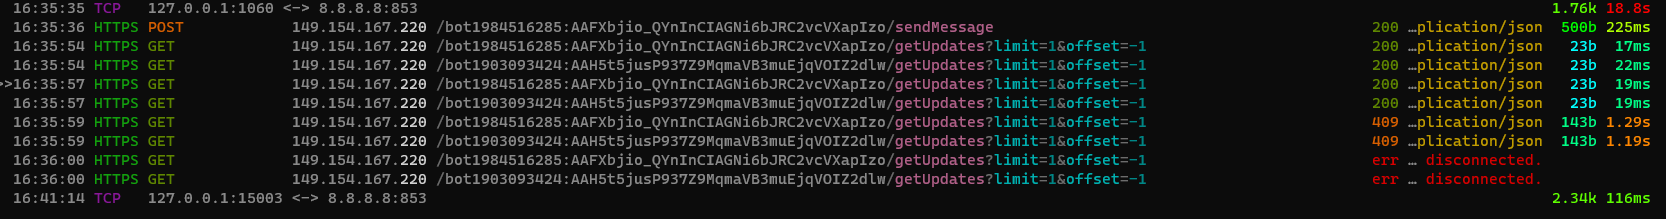
\includegraphics[width=1\textwidth]{requests made.png}
    \caption{Request list}
    \label{rafael-requestlist}
\end{figure}

\subsubsection{Wireshark analysis}

VirusTotal indicated that the malicious application made a connection to two IP addresses, one of these IP addresses already turned out to be Telegram.
However, the other was not detected using the HTTP Proxy.
Wireshark was used to confirm that no connection was actually being made. Wireshark did not detect any connections to the IP visible in VirusTotal.

\subsubsection{Reconnaissance}

An analysis was done on both IP address, the first IP that was found was already discovered to be from telegram.
\href{https://www.shodan.io/host/149.154.167.220}{Shodan} confirmed this thought.

\href{https://www.shodan.io/host/142.250.31.188}{Shodan} revealed that the second IP was owned by Google LLC. This indicated that this IP was not very interesting.
It only had one open port, 443, which normally would contain the HTTPS protocol.
In this case however, it only returned a single \texttt{)} with the Unicode character, EOT (End of transmission).